\chapter{The ScienceIE Task: Evaluation}

\begin{table}
	\centering
	\begin{tabular}{ c | C{2.7cm} | C{2.7cm} | C{2.2cm} | C{2.2cm} }
		\multirow{2}{*}{\textbf{Subtask}} &\multicolumn{2}{c|}{\textbf{ScienceIE}} &\multicolumn{2}{c}{\textbf{This Report}} \\
		& \textbf{Individual \newline Best / Average} & \textbf{End-To-End \newline Best / Average} & \textbf{Individual \newline Best} & \textbf{End-To-End \newline Best} \\
		\hline
		Key Phrase Extraction & 0.56 / 0.38 & 0.56 / 0.38 & 0.2 & 0.2 \\
		Key Phrase Classification & 0.67 / 0.57 & 0.44 / 0.26 & 0.55 & 0.11 \\
		Relation Extraction & 0.64 / 0.43 & 0.28 / 0.07 & 0.1 & 0.02 \\
		Overall & N/A & 0.43 / 0.25 & N/A & 0.11    
	\end{tabular}
	\caption[Summary of Results Evaluated With ScienceIE Scripts]{The best F1 scores achieved in this paper evaluated with the supplied ScienceIE scripts. This includes both tests for end-to-end data production, and individual subtask tests (where the gold standard data from the previous subtask is fed in). Summarised ScienceIE results are also included, extracted from the ScienceIE proceedings\cite{Augenstein2017}.}
	\label{table:scienceieresults}
\end{table}

With solution systems proposed for the various subtasks of ScienceIE, each were trained and their predictions on the ScienceIE test data made. Below are results where the algorithms have been tested end-to-end (where they are run through in order, with the data from one being passed to the next) and independently (where they are given the gold data as a starting point, and operate on that information). There is also some self evaluation conducted, to explore the effectiveness of evaluating under conditions of varying strictness.

A summary of evaluation using the ScienceIE scripts, which covers all subtasks using the best algorithms found within this paper, and also includes the ScienceIE scores for comparison, is presented in table \ref{table:scienceieresults}. These results will be discussed throughout this section.

\section{Subtask A - Key Phrase Extraction}

\subsection{Method 1: Support Vector Machine}

\begin{figure}[t]
	\includegraphics[width=\textwidth]{img/kpsvmresults.png}
	\caption[Key Phrase SVM Self Evaluation Through Iterations]{The key phrase SVM self evaluation results for varying strictness across iterations, where each iterations changes 1 thing. The coloured lines denote strictness as defined in table \ref{table:strictness}, with the legend assigning each colour to each strictness level. With each assignment, the darker of variant of the same colour is when the Google News (GN) Word2Vec model is used, and the lighter for when the Freebase (FB) model is used. Very strict evaluation was only created part way through development, so some early results are missing for that, but they would likely follow a similar patter to that of matching or \textit{strict} evaluation.}
	\label{figure:kpsvmresults}
\end{figure}

As described in the design section of this report, the SVM created for extracting key phrases began with a set of features which then underwent several iterations with other features and post processing being added. The full results, from start to finish showing each addition, can be seen in figure \ref{figure:kpsvmresults}.

The results of the initial SVM are interesting. The strict metric shows middling results below that of ScienceIE's average. However, the two more generous metrics are very high. This implies two good things: Firstly, as the \textit{inclusive} metric is high, it shows that while some unwanted information is being extracted, much of the key phrase data is been chosen. Furthermore, the \textit{generous} metric scoring not much higher implies that a lot of the other key phrases incorrectly extracted are just noise produced by the SVM rather than the gold key phrases with some missing information. This shows that the SVM isn't performing terribly as much of the required information is outputted, however, it has some overflowing of extra information which needs to be reduced. The redundant information could be removed by improvements to the SVM, as well as some post analysis and processing to remove extra, unwanted pieces of information, which is why the post processes discussed were developed and their analysis is to follow.

The Word2Vec features added generally slightly improved things across all metrics for at least one Word2Vec model. Oddly, while using the Google News model increased the score for the more generous two metrics, it negatively impacted the strict metric, reducing the F1 score by 6\% compared to the original score. The Freebase model was the opposite of this, although less significant differences were observed, as for the more generous metrics performance slightly degraded, and for the strict metric performance slightly improved. For this feature, it would imply Freebase was the best model to use as it did increase the results of the strictly measured predictions. 

The first post processing effect was then added: the TF-IDF filter. This gave all configurations minor improvements (the average F1 score rose by 0.01) as expected. 

Including the parse depth feature saw averagely 0.01 score improvements across the board as well. The graph showing progression also begins to include the very strict metric as well. This metric is in-line with how the ScienceIE evaluation works, matching both the key phrase string and position in the document. The result saw a 60\% score reduction compared to the, just string matching, strict metric when using both Freebase and Google News. This means the system is choosing useful pieces of information from the papers, but unfortunately roughly half of the key phrases chosen are not from the correct place in the text. 

Following this, the largest change to the SVM based key phrase extraction system happened; the inclusion of the \textit{sanitisation on creation} changes saw large improvements in F1 score - averagely 0.1 improvement for the Google News based strictly and very strictly evaluated tests. This was a very positive step, as the two generous metric scores didn't change very much. This mean that this post processing was effectively transforming a number of key phrases from being inclusive of the gold standard to matching the gold standard. 

Including the stop word flag feature again slightly improved things for the actual SVM performance, again averaging an increase of 0.01 F1 score.

The final change to the SVM process was to make the final changes to the key phrase creation sanitisation. While averagely this made no difference to the F1 results, for some cases it significantly damaged scores; namely when using the inclusive metric with the Freebase model, the F1 score dropped by almost 0.1. The Freebase model, under these presented set of features and processes, performs worse than the Google News model for all metrics aside from \textit{strict}, where the difference in F1 score is only 0.02. This change was still positive however, as it made the key phrases much more pleasant to look at. Cases such as ``support vector machine (svm'' were tidied up, and generally words were not missing end letters which was a problem from earlier in SVM's life (such as ``ncorporation'' missing the leading `i'). Furthermore, this last change saw an opportunity to quickly generate some synonyms for almost no cost. Using this method saw 14 synonyms correctly generated when processing the test data. 

From this, the best configuration can be seen to be when all proposed features and processing effects are used, with the Google News model being used for the Word2Vec features. Running this configuration and evaluating the predicted key phrase with the ScienceIE test scripts produces an overall F1 score of 0.2. This is perfectly in line with the self evaluation conducted under the strictest metric, which reinforces the self evaluation as trustworthy (as it got the correct score), and through that helps to validate claims drawn from other self evaluation metrics. 

\subsubsection{Experimenting With Longer Documents}
The ScienceIE proceeding paper SemEval 2017 \cite{Augenstein2017} was chosen to be tested in the key phrase extraction system. The SVM with all extensions and post processed was used to extract key phrases from the paper, and the results analysed. For this, the paper was manually converted from its PDF format to a text document, stripping all headings, footnotes, pre and post amble, leaving only the abstract and main content.

From the long paper, only 121 key phrases were extracted, with only 69 unique phrases. Furthermore, of the unique key phrases, many were very similar, only different because of line breaks, spaces or punctuation throughout the word (for example, ``scenario\_\_teams'' and ``scenario\-teams'', ``annotator'' and ``anno-tator''). There were 201 words across all 121 key phrases, meaning that most of the key phrases were very short (an average of 1.7 words per key phrase) which is quite low compared to the average 3 in the ScienceIE test data. 

Something that didn't happen was an overload of key phrases. While around triple the largest number of key phrases for a single document in the ScineceIE training set, given the length of the document, 121 is actually quite low. Only 5.7\% of the tokens in the document were labelled as a key phrase, which is significantly lower than the 36\% average in the ScienceIE training set.

In terms of the quality of the key phrases, there were some important pieces of information extracted (such as ``annotations of hypernym'', ``SVM'', ``scientific articles of the Computer Science''), but most were a single word which held little information. It repeatedly selected ``subtask'' and ``documents'', and while these are important to the document they are not necessarily key phrases of it. Aside from learning a little about the ScienceIE task, and the name of some of the teams attempting solutions, the extracted key phrases provide little information to help describe the actual content of the paper.

\subsection{Method 2: Clustering}
While the SVM method showed some reasonable results, unfortunately clustering was not as successful. 

A problem encountered during development was that not every word was in the Word2Vec vocabulary (the Google News model was used for this experiment), meaning not every word could be clustered. This is actually quite a major problem as, given the context of the words we'd like to cluster is scientific papers, many of these unusual words not in the corpus are likely part of the key words describing the key pieces of information in the paper. This limits the capability and robustness of the algorithm. The only thing that could be done was to continue clustering until we are left with one cluster with everything that can be clustered in, and a group of clusters with one element each, where those singular terms are not in the vocabulary of Word2Vec. This problem didn't occur for every test paper processed, but has shown some papers to have over 20 tokens that were excluded from the Word2Vec model. 

Next came the problem of how the clusters formed. Ideally, we would like to see the case where, for many iterations, many clusters are present with many items each. This could then be used to split the document into many clusters with a key phrase in each, taking the tokens at the centre of each cluster at a given level to be part of its own key phrase. What was generated instead was a pattern where, generally, two items clustered together which were there joined by a third item on the next iteration, then a fourth on the next, and so on, while no other tokens clustered together in other clusters. A visualisation of this is shown in figure \ref{figure:kpclusteringeg}, abstracted down to a few, rather than many items. This is significantly less useful, as a bunch of words are grouped together in a growing group, while all others are left on their own until they are included in this large group. Very occasionally, other clusters grew to have a few items rather than immediately join the large cluster, but this was rare to see and still not very useful to draw multiple key phrases from.

\begin{figure}
	\centering
	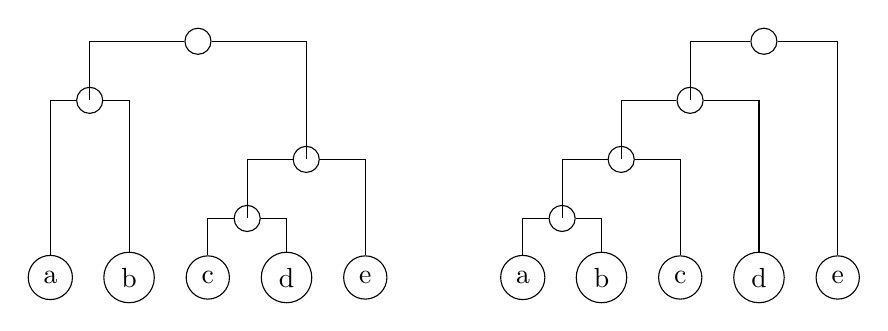
\begin{tikzpicture}[nodes={draw, circle}]
	\node (a) at (-4, 0) {a};
	\node (b) at (-3, 0) {b};
	\node (c) at (-2, 0) {c};
	\node (d) at (-1, 0) {d};
	\node (e) at (0, 0) {e};
	\node (ab) at (-3.5, 2.25) {};
	\node (cd) at (-1.5, 0.75) {};
	\node (cde) at (-0.75, 1.5) {};
	\node (all) at (-2.125, 3) {};
	
	\draw  (a) |- (ab);
	\draw  (b) |- (ab);
	\draw  (c) |- (cd);
	\draw  (d) |- (cd);
	\draw  (e) |- (cde);
	\draw  (cd.center) |- (cde);
	\draw  (ab.center) |- (all);
	\draw  (cde.center) |- (all);
	
	\node (a2) at (2 ,0) {a};
	\node (b2) at (3, 0) {b};
	\node (c2) at (4, 0) {c};
	\node (d2) at (5, 0) {d};
	\node (e2) at (6, 0) {e};
	\node (ab2) at (2.5, 0.75) {};
	\node (abc2) at (3.25, 1.5) {};
	\node (abcd2) at (4.125, 2.25) {};
	\node (all2) at (5.0625, 3) {};
	
	\draw  (a2) |- (ab2);
	\draw  (b2) |- (ab2);
	\draw  (c2) |- (abc2);
	\draw  (d2) |- (abcd2);
	\draw  (e2) |- (all2);
	\draw  (ab2.center) |- (abc2);
	\draw  (abc2.center) |- (abcd2);
	\draw  (abcd2.center) |- (all2);
	\end{tikzpicture}
	\caption[Visual Representation of Key Phrase Clustering]{Examples of hierarchical clustering on a set of items, \textit{a}, \textit{b}, \textit{c}, \textit{d} and \textit{e}, through to when they are all in the same cluster. The left drawing is an example of ideally what we would like to have seen. The right is a representation of what was very common generated.}
	\label{figure:kpclusteringeg}
\end{figure}

\section{Subtask B - Key Phrase Classification}

\begin{table}
	\centering
	\begin{tabular}{ C{2.5cm} | C{2cm} | C{2cm} | C{2cm} | C{2cm} | C{2cm} }
		\textbf{Word2Vec Model} & \textbf{Distance Metric} & \textbf{Default Class} & \textbf{Remove words?} & \textbf{Use many words?} & \textbf{Accuracy} \\
		\hline
		Google News & Average & Unknown & No & No & \textbf{47.90\%} \\
		Google News & Average & Unknown & Yes & No & \textbf{47.76\%} \\
		Google News & Average & Unknown & No & Yes & \textbf{45.47\%} \\
		Google News & Average & Unknown & Yes & Yes & \textbf{45.47\%} \\
		\textbf{Google News} & \textbf{Average} & \textbf{Material} & \textbf{No} & \textbf{No} & \textbf{54.58}\% \\
		Google News & Average & Material & Yes & No & \textbf{54.43\%} \\
		Google News & Average & Material & No & Yes & \textbf{52.14\%} \\
		Google News & Average & Material & Yes & Yes  & \textbf{52.14\%} \\
		Google News & Closest & Unknown & No & No & \textbf{46.05}\% \\
		Google News & Closest & Unknown & Yes & No & \textbf{45.96\%} \\
		Google News & Closest & Unknown & No & Yes & 44.05\% \\
		Google News & Closest & Unknown & Yes & Yes & 43.91\% \\
		Google News & Closest & Material & No & No & \textbf{52.73\%} \\
		Google News & Closest & Material & Yes & No & \textbf{52.63\%} \\
		Google News & Closest & Material & No & Yes & \textbf{50.73}\% \\
		Google News & Closest & Material & Yes & Yes & \textbf{50.58\%} \\
		Freebase & N/A & Unknown & N/A & N/A & 0.00\% \\
		Freebase & N/A & Material & N/A & N/A & 44.05\% \\
	\end{tabular}
	\caption[Word2Vec Classification Results]{The above table is the various configurations of the Word2Vec classifier, running with every possible configuration for the five parameters are listed. The result in bold line is the highest scoring configuration, with bold results being those above the baseline score of 44.05\% which is where every key phrase is simply classified as a \textit{material}. All Freebase results were not listed as there was no change in result other than for the \textit{default class} variable, so \textit{N/A} is present instead of each iteration of those variables. These results are based on classifying all 2052 ScienceIE key phrase test data points.}
	\label{table:classresults}
\end{table}

Key phrase classification under the outlined Word2Vec classifier was quick to execute. After the initial, one time per system boot wait for the Word2Vec model to be loaded into memory, the actual calculations required are very fast to execute, giving this classifier a very high throughput.

In terms of result, it can be seen that several configurations allow for over 50\% of the key phrases to be classified correctly. The full range of results for each configuration can be seen on table \ref{table:classresults}.

The obvious thing to note here is that all tests under Freebase without a default class have a 0\% accuracy (i.e. it didn't classify any key phrase correctly). With a little investigation, if all key phrases were labelled as a \textit{material}, the accuracy would be 44\% - which is what was achieved by all configurations with the Freebase model and a default classification of \textit{material}. Therefore, Freebase clearly isn't an effective vocabulary for working with scientific publications, seemingly containing none of the supplied words. 

When using the Google News model, things are more interesting. Generally, using this model a decent accuracy can be achieved, even without the support of a default classification. This shows the model does include many of the terms used in the publications presented. In terms of distance metric, \textit{average} was slightly better; it was part of the best configuration (scoring 54.6\%), and also the average of all of the \textit{average} distance configurations was 2\% higher than the average of the \textit{closest} configurations (50\% and 48\% respectively).

The configuration change that made the least difference was whether or not the stop words were removed. This saw changes, averagely, of 0.1\% when comparing two configurations differing in only whether these words were removed. When some words were not removed the algorithm performed better, indicating that these words are more important than first thought for deciding class. This may be down to the edge cases discussed such as ``He'' or similar which, despite being a stop word, we would want to keep.

Using various words when finding similarity decreased the accuracy of classification, and was the largest detrimental parameter. When using many words to find similarity, accuracy decreased an average of 2.2\% (50.3\% down to 48.1\%). This means the position of the target classes in the Word2Vec model are likely quite accurate when compared to words that can be used in a similar context.

Using the best configuration found my testing within this paper, evaluating this classifier through the ScienceIE scripts gives an F1 score of 0.55 when evaluated individually (given the gold standard key phrases). This isn't a bad score, as it almost matches the average ScienceIE F1 score for this section done independently.

\subsection*{Other Experimentation}
While working on key phrase classification, having seen some decent results produced by the SVM created in subtask A, a short experiment was conducted to see how well using position in a document could be used to determine classification.

The process of trying this was very simple: re-purpose the subtask A SVM (with all extensions) code to label training data according to class rather than to key phrase. Two versions of this were attempted:

\begin{itemize}
	\item The SVM is given 4 different labels, one for each classification and one for no classification (i.e. not part of a key phrase).
	\item 3 different SVMs were trained, each only having one classification labelled.
\end{itemize}

This was not expected to perform well as semantics are important for classification, which this SVM has little of.

As expected, performance was poor, with F1 scores for both versions being less than 0.1. This confirms that the position of tokens is not (very) useful in classifications. It may have been interesting to try again leaving out non key phrase tokens from the training data generated for the SVM to learn from, but these low results didn't encourage further study into this idea when other, more efficient and productive concepts were being worked on.

\section{Subtask C - Relation Extraction}

Both SVMs concepts were tested and the results for the hyponym and synonym variants combined for full evaluation.

\begin{table}
	\centering
	\begin{tabular}{ c | c | c | c | c }
		\textbf{SVM Model} & \textbf{Vector Generation} & \textbf{True Positives} & \textbf{False Positives} & \textbf{F1 Score} \\
		\hline
		\textit{Many Features} & All tokens included & 13 & 84 & \textbf{0.09} \\
		\textit{Many Features} & Root noun selected & 2 & 28 & 0.02 \\
		\textit{Many Features} & Stop words removed & 0 & 0 & 0 \\
		\textit{Few Features} & All tokens included & 0 & 0 & 0 \\
	\end{tabular}
	\caption[Relation Extraction Specific Results]{Results from doing relation extraction with the proposed SVMs. The results are calculated after the relations extracted by the hyponym and synonym SVMs are combined. The \textit{vector generation} column described how a vector for a key phrase was found.}
	\label{table:relresults}
\end{table}

As presented in summary table \ref{table:scienceieresults}, the best overall results for this synonym extraction was an F1 score of 0.1\%. This was from using the \textit{many features} SVM with the vectors from each token in a key phrase being used to calculate a key phrases total vector. A more detailed breakdown of how well each configuration performed can be seen in table \ref{table:relresults}. 

From this table is it clear to see that the \textit{many features} SVM concept performed better than the \textit{few features}. While the hope was to allow the SVM to work on information with a lower complexity to help it find a better fitting hyperplane, this clearly hasn't worked as it didn't pick any relations at all; compared to \textit{many features} with the same vector generation, which chose a total of 101 relations. 

In terms of the different methods of generating vectors for key phrases, keeping all of the information in the key phrase appears to be the best method. Most true positives where found when all tokens are kept, while less true positives came from where the root nouns are selected, and no true positives were found when stop words words were removed. This mirrors what happened in subtask B, where potentially unimportant information was removed and a decrease in the quality of results is observed; although it is more noticeable here given it is the difference between some and no relations being extracted (there was only a 0.1\% change in subtask B's results).

Furthermore, while leaving more important information in the key phrase for vector generation did improve the system performance, the false positives increases a large amount as well. Using all tokens is still the best method however, as selecting just the root noun saw 14 times more false positive results than true positive; compared to 6 times when using all tokens. Not excluding data clearly improves the system accuracy, and increases the F1 score.

\section{Discussion}
This paper set out to provide a set of solutions to the ScienceIE task and its subtasks. Considering the summary presented in table \ref{table:scienceieresults}, these experimental systems have performed in a satisfactory manor. 

The key phrase extraction using a range of features in a support vector machine and some effective post processing achieved reasonable results considering, if we ignore the location of the key phrase extractions, a maximum F1 score of 0.36 which is very close the to average at ScienceIE. For comparisons sake, it would be very interesting to run the same analysis on the results produced at ScienceIE, to see if the best teams realistically came very close to extracting 100\% of the required information (if the position of key phrases could be ignored, and potentially a little bit of extra information allowed). Clustering with Word2Vec was not successful, as not useful clusters could be formed. 

Given the extraction examination completed on a much longer document, this algorithm is not suitable for long documents. This places the algorithm's purpose perhaps at being used to extract information from abstracts or similar, which should hold several key points from the paper. This can then be used to help identify papers for reading further into.

The key phrase classification produced good results, again being very close to the average at ScienceIE. While the Freebase Word2Vec model did not serve this use well, the Google News model did a very good job of classifying key phrases, producing comparable results with or without a default classification to give if it couldn't understand a key token. 

Finally, the relation extraction did not perform very well, even when attempting just hyponym or synonym extraction. In fact, the one simple rule included in the post processing for subtask A produced 1 more correct synonym than any relation SVM did during testing with gold standard data as an input. From this, unfortunately using just Word2Vec as a basis for a SVM feature set cannot be recommended, as it has very poor performance under these conditions. It is believe, however, that part of this is because of the lack of testing data as input, given there were many examples given to the SVM of what a relationship didn't look like, where there were few examples of what the relationships did look like.

\subsection{Improvements}
From this, a range of improvements and extensions could be applied:
\begin{itemize}
	\item \textbf{A more appropriate Word2Vec model.} Word2Vec was used in all three subtasks, but unfortunately only two models were tested with the systems, and neither had the context of scientific papers. If a system was created to crawl the internet fetching many scientific publications and have them all processed by Word2Vec, there may be a potential for a more suitable model to be created. Not only would the vocabulary be laid out in vector space in a way that should likely fit the testing data presented here better, but more of the tokens in this testing data should also appear in the model, which would improve things significantly for a start. This would likely impact the solution to subtask B the most, although it may significantly help the clustering attempts in subtask A if it can produce a more balanced progression clustering.
	\item \textbf{Expansion of key phrase SVM features.} If future work was to continue on the SVM created in subtask A, a way that is likely to produce better results is to include more features about each token. Specifically:
	\begin{itemize}
		\item Features giving more information about surrounding key phrase tokens (for example more information about recent key phrase tokens, information about overall key phrases so far for the given document),
		\item The Word2Vec distance to the previous token (in an attempt to string together related tokens),
		\item More lexical or semantic information about the current phrase.
	\end{itemize}
	\item \textbf{More training time and memory capacity for parameter tuning.} Time and memory limitations didn't allow for much more training time to be given to the \textit{many features} SVM, but potentially an increased \textit{C} value may help to find a hyperplane which could work better. For the key phrase SVM, while the parameters tested in cross validation seemed to plateau, further investigation may have revealed increased performance.
	\item \textbf{Better data for training the relation SVMs.} As alluded to above, give the relation SVMs training data which includes a higher percentage of actual relations cases. This could be done through adding more papers with relations in, or removing some or all papers without any relations in.
	\item \textbf{Experiment with full scientific publications.} While this subject was touched upon briefly in this report, working with full publications rather than short extracts would help contribute to the problem of information retrieval, which currently needs development in the context of long documents. Clearly, the algorithm proposed here is not useful when applied to full publications (in the limited testing done), as no meaningful information is extracted beyond what the title of the document should give. Potentially, the strongest algorithms presented produced at ScienceIE could be recreated, tested and altered to work with longer papers.
	\begin{itemize}
		\item One method that may be worth exploring, given the algorithms proposed here are targeting short documents, is that processing could be completed on individual paragraphs producing many key phrases for a document. Then a system could be developed to look at the generated key phrases for each paragraph and choose a selection to represent the entire paper.
	\end{itemize}
\end{itemize}
